%%%%%%%%%%%%%%%%%%%%%%%%%%%%%%%%%%%%%%%%%%%%%%
%
%		My Thesis
%
%		EDOC Template
%		2011
%
%%%%%%%%%%%%%%%%%%%%%%%%%%%%%%%%%%%%%%%%%%%%%%


%%%%%%%%%%%%%%%%%%%%%%%%%%%%%%%%%%%%%%%%%%%%%%
%
%		Thesis Settings
%
%		EDOC Template
%		2011
%
%%%%%%%%%%%%%%%%%%%%%%%%%%%%%%%%%%%%%%%%%%%%%%
\documentclass[a4paper,12pt,fleqn,print,oneside]{book}

\usepackage[T1]{fontenc}
\usepackage[utf8]{inputenc}
\usepackage[english, vietnamese]{babel}
%\usepackage{bookman}

%%%%%%%%%%%%%%%%%%%%%%%%%%%%%%%%%%%%%%%%%%%%%%%
%% EDOC THESIS TEMPLATE: Variant 1.0 -> Latin modern, large text width&height
%%%%%%%%%%%%%%%%%%%%%%%%%%%%%%%%%%%%%%%%%%%%%%%
%\usepackage{lmodern}
%\usepackage[a4paper,top=22mm,bottom=28mm,inner=35mm,outer=25mm]{geometry}
%%%%%%%%%%%%%%%%%%%%%%%%%%%%%%%%%%%%%%%%%%%%%%%

%%%%%%%%%%%%%%%%%%%%%%%%%%%%%%%%%%%%%%%%%%%%%%
% EDOC THESIS TEMPLATE: Variant 2.0 -> Utopia, Gabarrit A (lighter pages)
%%%%%%%%%%%%%%%%%%%%%%%%%%%%%%%%%%%%%%%%%%%%%%
%\usepackage[libertine,cmintegrals,cmbraces,vvarbb]{newtxmath}
\usepackage{mathpazo}
%\usepackage{utopia} % Utopia font-typesetting including mathematical formula compatible with newer TeX-Distributions (>2010)
%\usepackage{pia} % on older systems -> use this package instead of fourier in combination with mathdesign for better looking results
%\usepackage[adobe-utopia]{mathdesign}
\setlength{\textwidth}{146.8mm} % = 210mm - 37mm - 26.2mm
\setlength{\oddsidemargin}{11.6mm} % 37mm - 1in (from hoffset)
\setlength{\evensidemargin}{0.8mm} % = 26.2mm - 1in (from hoffset)
\setlength{\topmargin}{-2.2mm} % = 0mm -1in + 23.2mm 
\setlength{\textheight}{221.9mm} % = 297mm -29.5mm -31.6mm - 14mm (12 to accomodate footline with pagenumber)
\setlength{\headheight}{14pt}
%%%%%%%%%%%%%%%%%%%%%%%%%%%%%%%%%%%%%%%%%%%%%%


\usepackage[T1]{fontenc}
\usepackage{lmodern}
%\setlength{\parindent}{0pt}

\usepackage{setspace} % increase interline spacing slightly
\setstretch{1.1}

\makeatletter
\setlength{\@fptop}{0pt}  % for aligning all floating figures/tables etc... to the top margin
\makeatother


\usepackage{graphicx,xcolor}
\graphicspath{{images/}}

%\usepackage{subfig}
\usepackage{booktabs}
\usepackage{lipsum}
\usepackage{microtype}
\usepackage{url}
\usepackage[final]{pdfpages}

\usepackage{fancyhdr}
\renewcommand{\sectionmark}[1]{\markright{\thesection\ #1}}
\pagestyle{fancy}
	\fancyhf{}
	\renewcommand{\headrulewidth}{0.4pt}
	\renewcommand{\footrulewidth}{0pt}
	\fancyhead[OR]{\bfseries \nouppercase{\rightmark}}
	\fancyhead[EL]{\bfseries \nouppercase{\leftmark}}
	\fancyfoot[EL,OR]{\thepage}
\fancypagestyle{plain}{
	\fancyhf{}
	\renewcommand{\headrulewidth}{0pt}
	\renewcommand{\footrulewidth}{0pt}
	\fancyfoot[EL,OR]{\thepage}}
\fancypagestyle{addpagenumbersforpdfimports}{
	\fancyhead{}
	\renewcommand{\headrulewidth}{0pt}
	\fancyfoot{}
	\fancyfoot[RO,LE]{\thepage}
}

\usepackage{listings}
\lstset{language=[LaTeX]Tex,tabsize=4, basicstyle=\scriptsize\ttfamily, showstringspaces=false, numbers=left, numberstyle=\tiny, numbersep=10pt, breaklines=true, breakautoindent=true, breakindent=6pt}

\usepackage{hyperref}
\hypersetup{pdfborder={0 0 0},
	colorlinks=true,
	linkcolor=black,
	citecolor=black,
	urlcolor=black}
\urlstyle{same}

\makeatletter
\def\cleardoublepage{\clearpage\if@twoside \ifodd\c@page\else
    \hbox{}
    \thispagestyle{empty}
    \newpage
    \if@twocolumn\hbox{}\newpage\fi\fi\fi}
\makeatother \clearpage{\pagestyle{plain}\cleardoublepage}


%%%%% CHAPTER HEADER %%%%
\usepackage{color}
\usepackage{tikz}
\usepackage[explicit]{titlesec}
\newcommand*\chapterlabel{}
%\renewcommand{\thechapter}{\Roman{chapter}}
\titleformat{\chapter}[display]  % type (section,chapter,etc...) to vary,  shape (eg display-type)
	{\normalfont\bfseries\Huge} % format of the chapter
	{\gdef\chapterlabel{\thechapter\ }}     % the label 
 	{0pt} % separation between label and chapter-title
 	  {\begin{tikzpicture}[remember picture,overlay]
    \node[yshift=-8cm] at (current page.north west)
      {\begin{tikzpicture}[remember picture, overlay]
        \draw[fill=black] (0,0) rectangle(35.5mm,15mm);
        \node[anchor=north east,yshift=-7.2cm,xshift=34mm,minimum height=30mm,inner sep=0mm] at (current page.north west)
        {\parbox[top][30mm][t]{15mm}{\raggedleft $\phantom{\textrm{l}}$\color{white}\chapterlabel}};  %the black l is just to get better base-line alingement
        \node[anchor=north west,yshift=-7.2cm,xshift=37mm,text width=\textwidth,minimum height=30mm,inner sep=0mm] at (current page.north west)
              {\parbox[top][30mm][t]{\textwidth}{\color{black}#1}};
       \end{tikzpicture}
      };
   \end{tikzpicture}
   \gdef\chapterlabel{}
  } % code before the title body

\titlespacing*{\chapter}{0pt}{50pt}{30pt}
\titlespacing*{\section}{0pt}{12pt}{*0}  % 13.2pt is line spacing for a text with 11pt font size
\titlespacing*{\subsection}{0pt}{12pt}{*0}
\titlespacing*{\subsubsection}{0pt}{12pt}{*0}

\newcounter{myparts}
\newcommand*\partlabel{}
\titleformat{\part}[display]  % type (section,chapter,etc...) to vary,  shape (eg display-type)
	{\normalfont\bfseries\Huge} % format of the part
	{\gdef\partlabel{\thepart\ }}     % the label 
 	{0pt} % separation between label and part-title
 	  {\setlength{\unitlength}{20mm}
	  \addtocounter{myparts}{1}
	  \begin{tikzpicture}[remember picture,overlay]
    \node[anchor=north west,xshift=-65mm,yshift=-6.9cm-\value{myparts}*20mm] at (current page.north east) % for unknown reasons: 3mm missing -> 65 instead of 62
      {\begin{tikzpicture}[remember picture, overlay]
        \draw[fill=black] (0,0) rectangle(62mm,20mm);   % -\value{myparts}\unitlength
        \node[anchor=north west,yshift=-6.1cm-\value{myparts}*20mm,xshift=-60.5mm,minimum height=30mm,inner sep=0mm] at (current page.north east)
        {\parbox[top][30mm][t]{55mm}{\raggedright \color{white}Part \partlabel $\phantom{\textrm{l}}$}};  %the phantom l is just to get better base-line alingement
        \node[anchor=north east,yshift=-6.1cm-\value{myparts}*20mm,xshift=-63.5mm,text width=\textwidth,minimum height=30mm,inner sep=0mm] at (current page.north east)
              {\parbox[top][30mm][t]{\textwidth}{\raggedleft \color{black}#1}};
       \end{tikzpicture}
      };
   \end{tikzpicture}
   \gdef\partlabel{}
  } % code before the title body
 
 
\usepackage{lastpage}
 
%\fancyhead[R]{
%	\begin{tabular}{l}
%		\tiny \bf \\
%		\tiny \bf 
%	\end{tabular}  }

%\fancyfoot{} % clear all footer fields
%\fancyfoot[R]{\ttfamily {\thepage}}
%\fancyfoot[L]{\scriptsize \ttfamily LUẬN VĂN TỐT NGHIỆP - Niên khóa 2014-2018}
%\fancyfoot[R]{\scriptsize \ttfamily Trang {\thepage}/\pageref{LastPage}}
%\renewcommand{\headrulewidth}{0.3pt}
%\renewcommand{\footrulewidth}{0.3pt}

\usepackage{amsmath}
% Fix the problem with delimiter size caused by fourier and amsmath packages.
\makeatletter
\def\resetMathstrut@{%
  \setbox\z@\hbox{%
    \mathchardef\@tempa\mathcode`\(\relax
      \def\@tempb##1"##2##3{\the\textfont"##3\char"}%
      \expandafter\@tempb\meaning\@tempa \relax
  }%
  \ht\Mathstrutbox@1.2\ht\z@ \dp\Mathstrutbox@1.2\dp\z@
}
\makeatother


%%%%%%%%%%%%%%%%%%%%%%%%%%%%%%%%%%%%%%%%%%%%%%
%
%		Thesis Settings
%		Custom settings
%
%		2011
%
%%%%%%%%%%%%%%%%%%%%%%%%%%%%%%%%%%%%%%%%%%%%%%

%
%   Use this file for your own custom packages, command-definitions, etc...
%


% the following lines are for creating a simplified TO-DO box. However since boites is not per default installed with all latex-distributions, we have removed this example again
% if you want to use it and do not have "boites" installed, you can get it from here: http://www.ctan.org/tex-archive/macros/latex/contrib/boites
%
%\usepackage{boites,boites_exemples}
%\newcommand{\todolist}[1]{\begin{boiteepaisseavecuntitre}{TO DO in this chapter} #1 \end{boiteepaisseavecuntitre}}  % creates a little box
% %\newcommand{\todolist}[1]{}  % to be used when to do is not to be printed
\usepackage[numbers]{natbib}
\bibliographystyle{IEEEtranN}
\usepackage[noabbrev, nameinlink]{cleveref}
\usepackage{pdfpages}
\usepackage{enumitem}
\usepackage{textcomp}
\usepackage{pifont}
\usepackage{tabto}
\usepackage{amssymb}
\usepackage{hyperref}
\usepackage{booktabs}
\usepackage{graphicx}
\usepackage{array}
\usepackage{pdflscape}
%\usepackage{subcaption}
\usepackage{subfig}
\usepackage{forest}

\makeatletter
\renewcommand*\l@figure{\@dottedtocline{1}{1em}{3.2em}}
\makeatother
  % place your custom packages, etc... in this file!
%\input{thesis-info.tex}

%%%%%%%%%%%%%%%%%%%%%%%%%%%%%%%%%%%%%%%%%%%%%%
%%%%% HEAD: Book-Begin
%%%%%%%%%%%%%%%%%%%%%%%%%%%%%%%%%%%%%%%%%%%%%%
\begin{document}
\frontmatter
%\begin{titlepage}
%\begin{center}
%%\large
%\sffamily
%
%
%\null\vspace{2cm}
%{\huge A survey of various data dissemination schemes for Vehicular Ad-hoc NETwork} \\[24pt] 
%\textcolor{gray}{\small{THIS IS A TEMPORARY TITLE PAGE \\ It will be replaced for the final print by a version \\ provided by the service academique.}}
%    
%\vfill
%
%\begin{tabular} {cc}
%\parbox{0.3\textwidth}{\includegraphics[width=4cm]{images/epfl}}
%&
%\parbox{0.7\textwidth}{%
%	Thèse n. 1234 2011\\
%	présenté le 12 Mars 2011\\
%	à la Faculté des Sciences de Base\\
%	laboratoire SuperScience\\
%	programme doctoral en SuperScience\\
%%
%%	ÉCOLE POLYTECHNIQUE FÉDÉRALE DE LAUSANNE\\
%	École Polytechnique Fédérale de Lausanne\\[6pt]
%	pour l'obtention du grade de Docteur ès Sciences\\
%	par\\ [4pt]
%	\null \hspace{3em} Paolino Paperino\\[9pt]
%%
%\small
%acceptée sur proposition du jury:\\[4pt]
%%
%    Prof Name Surname, président du jury\\
%    Prof Name Surname, directeur de thèse\\
%    Prof Name Surname, rapporteur\\
%    Prof Name Surname, rapporteur\\
%    Prof Name Surname, rapporteur\\[12pt]
%%
%Lausanne, EPFL, 2011}
%\end{tabular}
%\end{center}
%\vspace{2cm}
%\end{titlepage}

\begin{titlepage}
	%
\includepdf{head/cover.pdf}
\thispagestyle{empty}
\begin{center}
	\begin{large}
		\textbf{Đại học Quốc gia Thành phố Hồ Chí Minh}
	\end{large} \\
	\begin{large}
		\textbf{Trường Đại học Bách Khoa}
	\end{large} \\
	\begin{large}
		\textbf{Khoa Khoa học và Kỹ thuật Máy tính}
	\end{large} \\
	\textbf{--------------------  *  ---------------------}\\[1.2cm]
	
	\begin{center}
		
\includegraphics[scale=.2]{images/logo.png}\\[1.0cm]
	\end{center}
	
	{\fontsize{23pt}{1}\selectfont \textbf{Đề Cương Luận Văn}}\\[1.5cm]
	
	{\fontsize{24pt}{1}\selectfont \textbf{Đề tài:} Nghiên cứu và xây dựng giải pháp
		tích hợp giám sát hệ thống và quản trị
		mạng dùng trong các Data-Center}\\[1.75cm]
\end{center}

\hspace{2cm} Hội đồng \hspace{72pt} :  \hspace{5pt} \textbf{\parbox[t]{10cm}{
		Kỹ Thuật Máy Tính
}} 

\hspace{2cm} Giáo viên hướng dẫn \hspace{14pt} :  \hspace{4pt} \textbf{\parbox[t]{8cm}{
		TS. Nguyễn Lê Duy Lai
}} 

\hspace{2cm} Giáo viên phản biện \hspace{18pt} :  \hspace{4pt} \textbf{\parbox[t]{8cm}{
		Tên GV Phản Biện
}} \\


\hspace{2cm} Nhóm sinh viên thực hiện : \hspace{4pt}
\textbf{\parbox[t]{20cm}{
		Trương Quốc Huy \hspace{13pt} - 1511305\\
		Ngô Quốc Dũng \hspace{13pt} - 1510559\\
}}


\vspace{1.5cm}
%	\vspace{1.75cm}
\begin{center}
	%{\fontsize{20pt}{1} TP Hồ Chí Minh}\\
	{\fontsize{20pt}{1} \today}
\end{center}

\end{titlepage}




\cleardoublepage
\thispagestyle{empty}


\vspace*{3cm}

\begin{raggedleft}
    	I think, therefore I am;\\
     --- René Descartes\\
\end{raggedleft}

\vspace{4cm}




\setcounter{page}{0}
\chapter*{Lời cam đoan}
\markboth{Lời cam đoan}{Lời cam đoan}
\addcontentsline{toc}{chapter}{Lời cam đoan}
\vspace{1.0cm}
Nhóm cam đoan mọi điều được ghi trong báo cáo, cũng như mã nguồn là do nhóm tự thực hiện - trừ các kiến thức tham khảo có trích dẫn cũng như mã nguồn mẫu do chính nhà sản xuất cung cấp, hoàn toàn không sao chép từ bất cứ nguồn nào khác. Nếu lời cam đoan trái với sự thật, nhóm xin chịu mọi trách nhiệm trước Khoa và Nhà trường.
\begin{flushright}
Nhóm sinh viên thực hiện đề tài 
\end{flushright}


\bigskip
 
%\noindent\textit{Lausanne, 12 Mars 2011}
%\hfill D.~K.

\chapter*{Lời cảm ơn}
\markboth{Lời cảm ơn}{Lời cảm ơn}
\addcontentsline{toc}{chapter}{Lời cảm ơn}
\onehalfspacing
\vspace{1.0cm}
Sau bốn năm theo học tại khoa Khoa học Kĩ thuật Máy tính trường Đại học Bách khoa TP. Hồ Chí Minh, em đã được áp dụng tất cả những kiến thức đã học để thực hiện luận văn tốt nghiệp, đề tài cuối cùng mang tính quyết định kết quả học tập và quá trình tốt nghiệp.\\

Em xin chân thành cảm ơn quý thầy cô trong Khoa đã mang đến những kiến thức bổ ích trong suốt quãng đời sinh viên, đặc biệt là thầy Phạm Hoàng Anh đã giúp đỡ em trong quá trình thực hiện cũng như quá trình hoàn thiện luận văn. Em cũng gửi lời cảm ơn đến một số bạn bè trong Khoa đã hỗ trợ giúp em tiết kiệm được thời gian tìm hiểu đề tài. \\

Em đã cố gắng hết sức để tránh các sai sót, nhưng nếu có phát hiện thì mong quý thầy cô góp ý để em càng hoàn thiện đề tài hơn. Cuối cùng em xin gửi lời chúc sức khỏe và cảm ơn chân thành nhất.
\begin{flushright}
 Nhóm sinh viên thực hiện đề tài 
\end{flushright}

\bigskip
 
%\noindent\textit{Lausanne, 12 Mars 2011}
%\hfill D.~K.

%\input{head/achievement}
% English abstract
\cleardoublepage
\chapter*{Tóm tắt}
%\markboth{Abstract}{Abstract}
\addcontentsline{toc}{chapter}{Tóm tắt} % adds an entry to the table of contents
\vspace{1.0cm}
Gần đây, khái niệm Cách mạng Công nghiệp 4.0 được nhắc đến nhiều trên truyền thông và mạng xã hội. Cùng với đó là những hứa hẹn về cuộc đổi đời của các doanh nghiệp tại Việt Nam nếu đón được làn sóng này. Cách mạng Công nghiệp 4.0 sẽ diễn ra trên 3 lĩnh vực chính gồm Công nghệ sinh học, Kỹ thuật số và Vật lý. Những yếu tố cốt lõi của Kỹ thuật số sẽ là: Trí tuệ nhân tạo (AI), Vạn vật kết nối - Internet of Things (IoT) và dữ liệu lớn (Big Data)\cite{cmcn}. Trong đó IoT sẽ đảm nhiệm việc kết nối, thu nhập thông tin từ các thiết bị và vật dụng tạo nên Big Data, còn AI sẽ đảm nhiệm việc xử lý chúng.\\

Hiện nay các doanh nghiệp tham gia phát triển các hệ thống IoT sử dụng rất nhiều chuẩn kết nối khác nhau, có những chuẩn quen thuộc với đa số mọi người như WiFi, Ethernet, Bluetooth; cũng có những chuẩn thuộc dạng \lq\lq{}chuyên ngành\rq\rq{} như ZigBee, LoRa, Xbee, RFID. Mỗi chuẩn đều có những ưu nhược điểm riêng và phù hợp với các ứng dụng cụ thể.\\

Trong đề tài này, nhóm sẽ thảo luận về giao thức Bluetooth Mesh, một giao thức mạng được phát triển dựa trên chuẩn giao tiếp Bluetooth. Bluetooh Mesh là một chuẩn ra đời sau, khá mới so với những chuẩn khác nên khả năng chiếm giữ thị trường còn hạn chế. Tuy nhiên với những ưu điểm đầy hứa hẹn của mình, Bluetooh Mesh sẽ nhanh chóng thay đổi bộ mặt của lĩnh vực IoT.\\

Ngoài việc tổng hợp một số nghiên cứu của nhóm về nguyên lý hoạt động của Bluetooh Mesh để làm tài liệu tham khảo cho các khóa sau, nhóm còn tiến hành thử nghiệm hiện thực một ứng dụng đơn giản để chứng minh tiềm năng của Bluetooh Mesh. Ứng dụng bao gồm việc thu thập dữ liệu và cập nhật lên cloud thông qua mạng GPRS.


\vskip0.5cm
%put your text here


%\endgroup			
%\vfill


\tableofcontents
\pdfbookmark{\contentsname}{Mục lục}
\cleardoublepage
\phantomsection
\addcontentsline{toc}{chapter}{Mục Lục Hình} % 
\addcontentsline{toc}{chapter}{Danh Sách Bảng} %
adds an entry to the table of contents
\listoffigures
\cleardoublepage
\phantomsection
%\addcontentsline{toc}{chapter}{List of tables} % adds an entry to the table of contents
%\listoftables
%\cleardoublepage
%\phantomsection
\newcommand{\abbrlabel}[1]{\makebox[3cm][l]{\textbf{#1}\ \dotfill}}
\newenvironment{abbreviations}{\begin{list}{}{\renewcommand{\makelabel}{\abbrlabel}}}{\end{list}}

\chapter*{Thuật ngữ \& từ viết tắt}
\thispagestyle{empty}
\pagestyle{empty}
\addcontentsline{toc}{chapter}{Thuật ngữ \& từ viết tắt}
\vspace{1.0cm}
\begin{abbreviations}
	\item[AES] Advanced Encryption Standard 
	\item[BLE] Bluetooth Ligh Energy
	\item[BR/EDR] Basic Rate/Enhanced Data Rate 
	\item[CBC-MAC] Cipher Block Chaining Message Authentication Code
	\item[CCM] Counter with CBC-MAC
	\item[Cloud] Trong phạm vi đề tài, dùng để chỉ nơi lưu trữ dữ liệu trên internet
	\item[CMAC] Cipher-based Message Authentication Code
	\item[ECDH] Elliptic-curve Diffie–Hellman
	\item[GPRS] General Packet Radio Service
	\item[GSM] Global System for Mobile Communications
	\item[GUI] Graphical User Interface
	\item[IPv4] Internet Protocol version 4
	\item[IPv6] Internet Protocol version 6
	\item[LPN]  Low power node
	\item[Mesh] Mạng mesh là mạng mà các phần tử đều có kết nối với nhau
	\item[MITM] Man-in-the-midle: Chen giữa một kết nối nhằm mục đích xấu
	\item[Node] Node là một phần tử trong mạng mesh
	\item[OOB] Out-of-band
	\item[P2P] Peer-to-peer
	\item[TTL] Time To Live
	\item[Sleep] Trạng thái ngủ giúp tiết kiệm năng lượng
\end{abbreviations}
% your list of symbols here, if needed.


% space before each new paragraph according to the template guidelines.
%(needs to be after titlepage and frontmatter to keep the table of contents lists short)
\setlength{\parskip}{1em}


%%%%%%%%%%%%%%%%%%%%%%%%%%%%%%%%%%%%%%%%%%%%%%
%%%%% MAIN: The chapters of the thesis
%%%%%%%%%%%%%%%%%%%%%%%%%%%%%%%%%%%%%%%%%%%%%%
\mainmatter
\chapter{Giới thiệu đề tài}
\pagestyle{fancy}
Trong nền công nghệ phát triển như hiện nay, khi mà công nghệ chế tác các thiết
bị phần cứng đang đạt đến mức bão hòa ( ít đột biến ) thì bài toán về việc tối
ưu hóa ( tăng tính tương thích giữa thiết bị phần cứng và phần mềm, giảm tải
nguyên sử dụng, tăng hiệu suất hoạt động của hệ thống...) luôn được đặc biệt quan tâm. Để có hướng giải quyết bài
toán đó, trước hết chúng ta cần phải nắm rõ về hệ thống đó, biết được hệ thống
đang hoạt động ra sao, tốn bao nhiêu tài nguyên cho một tác vụ...

Từ đó, ta sẽ dễ dàng đưa ra được hướng giải quyết cho bài toán tối ưu. Trên thị
trường đã có các công cụ quản lí tài nguyên hệ thống như : Webmin, VirtualMin,
VestaCP, ISPconfig... hay công cụ quản trị mạng như : Nagios, Icinga, Zenoss,
Cisco Network Assistant... Tuy nhiên, gần như rất ít công cụ tích hợp quản trị tài nguyên và quản trị mạng lại với nhau, nếu có thì giá thành của nó vẫn còn khá cao. Bởi vậy việc cho ra một công cụ tối ưu giúp người giám sát hệ thống có được cái nhìn trực quan nhất về mọi mặt của hệ thống là điều hết sức cần thiết.

    \section{Nhiệm vụ cần đạt}
    \begin{itemize}
        \item Tìm hiểu các công việc liên quan đến việc giám sát, quản lý hệ thống và quản trị mạng.
        \item Tìm hiểu về các công cụ được sử dụng để giám sát hệ thống và quản trị mạng.
        \item Thiết kế mô hình ứng dụng, các tính năng và phương pháp tích hợp.
    \end{itemize}
   
\chapter{Nội dung thực hiện} \label{chap:theory}
    \section{Các công việc liên quan đến giám sát hệ
    	thống và quản trị mạng}
    	\begin{itemize}
    		\item Xác định, khắc phục sự cố, giải quyết và ghi lại các vấn đề kết nối và hiệu suất mạng.
    		\item Giám sát hiệu suất mạng và tối ưu hóa mạng để có tốc độ và tính sẵn sàng tối ưu.
    		\item Cài đặt, cấu hình và duy trì phần cứng mạng.
    		\item Triển khai, cấu hình và nâng cấp phần mềm mạng.
    		\item Triển khai và duy trì các hệ thống sao lưu và khôi phục khẩn cấp cho các máy chủ mạng quan trọng.
    		\item Giám sát tình hình hoạt động, tài nguyên của các thành phần trong hệ thống.
    		\item Quản trị quyền truy cập của người dùng vào những file nhạy cảm.
    		\item Quản lí user/group trên hệ thống.
    		\item Quản lí các phần mềm trên hệ thống.
    		\item Quản lý các công cụ bảo mật mạng,...
    	\end{itemize}

   	\section{Các công cụ được sử dụng để giám sát hệ thống và quản trị mạng}
   		\subsection{Giám sát hệ thống}
   		\textbf {Webmin}
   		
   		Chức năng nổi bật :
	   		\begin{itemize}
	   			\item Quản lí user/group trên hệ thống.
	   			\item Quản lí phần mềm trên hệ thống.
	   			\item Cấu hình thời gian cho hệ thống.
				\item Quản lí File.
				\item Thực thi lệnh linux.
	   		\end{itemize}
   	
   		Ưu nhược điểm :
   			\begin{itemize}
   				\item Miễn phí và có đầy đủ tính năng quan trọng.
   				\item Tương thích với WordPress.
   				\item Không thể tạo ra các host con để chia sẻ dùng chung.
   			\end{itemize}
   		\textbf {Virtualmin}
   		
   		Chức năng nổi bật :
   		\begin{itemize}
   			\item Quản lí giới hạn tài nguyên sử dụng.
   			\item Hỗ trợ backup và tự backup.
   			\item Giao diện thân thiện.
   			\item Quản lí user và tạo host.
   			\item Xem và quản lí các thiết lập về máy chủ, mạng.
   		\end{itemize}
   		
   		Ưu nhược điểm :
   		\begin{itemize}
   			\item Linh hoạt hơn, có thể định cấu hình, giao diện người dùng.
   			\item Có giao diện đẹp trên cả tablet và mobile.
   			\item Không thể tạo ra các host con để chia sẻ dùng chung.
   		\end{itemize}
   	
   		Hệ thống hỗ trợ :
   		\begin{itemize}
   			\item Ubuntu, CentOS/RHEL6 \& 7, Debian.
   		\end{itemize}
\chapter{Thiết kế ứng dụng}    
\section{Phần cứng} 
    Nhóm sử dụng Kit phát triển PCA10040 sử dụng SoC nRF52832 của Nordic Semiconductor, nguyên nhân nhóm chọn dùng Kit này là vì có hỗ trợ Bluetooth Mesh cùng với một số chức năng chính:
    \begin{itemize}
        \item Hỗ trợ ANT/ANT+, Bluetooth low energy, Bluetooth Mesh
        \item Buttons và LEDs on board
        \item I/O tương thích với chuẩn Arduino
        \item SEGGER J-Link OB debugger, có hỗ trợ debug ngoài
        \item Giao tiếp UART qua cổng COM ảo
        \item Lập rình drag-and-drop
        \item Hỗ trợ NFC-A listen mode
        \item Hỗ trợ mbed
    \end{itemize}
 
    
    \begin{figure}[h!]
    	\begin{center}
    		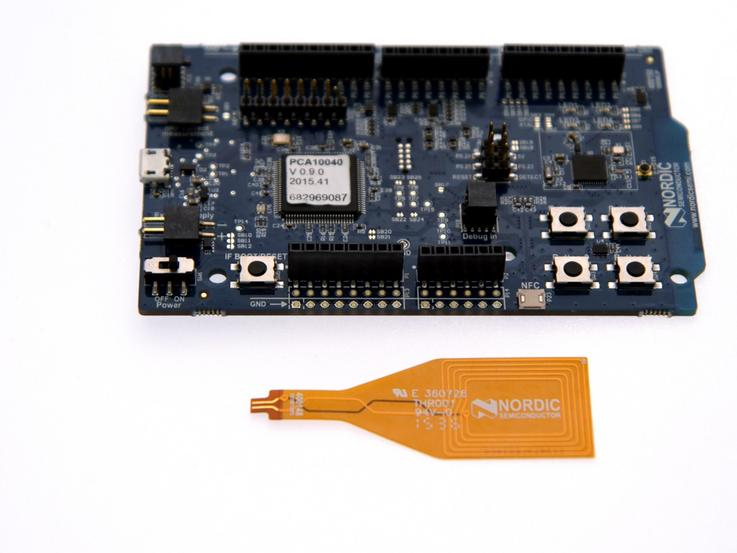
\includegraphics[scale=1.3]{images/nrf52-dk.jpg}
    		\caption{Hình ảnh KIT phát triển PCA10040}
    	\end{center}
    \end{figure}
    \newpage
    Module 3G SARA click cung cấp giải pháp cho các ứng dụng liên quan đến mạng điện thoại, sử dụng module 3.75G UMTS/HSPA SARA U-201 của U-blox. Module mang đầy đủ các chức năng như kết nối mạng, hỗ trợ TCP/UDP, HTTP và HTTPS, IPv4/IPv6, phát hiện nhiễu, đo cường độ tín hiệu,... 3G SARA hỗ trợ tốc độ gửi nhận dữ liệu lên đến 7.2 Mb/s (nhận) và 5.76 Mb/s (gửi), còn có thực hiện cuộc gọi 3G với chất lượng âm thanh tốt. Nguyên nhân nhóm chọn moule này để kết nối với cloud là vì đã từng dùng trong một dự án khác nên có kinh nghiệm với nó.

    \begin{figure}[h!]
    	\begin{center}
    		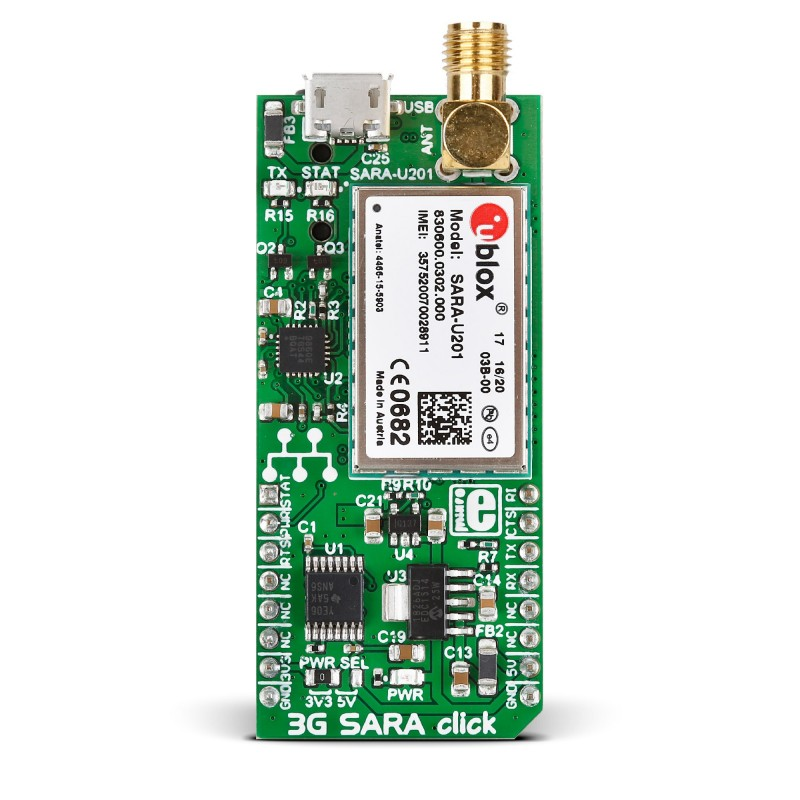
\includegraphics[scale=0.2, angle=90]{images/3g-sara-click.jpg}
    		\caption{Hình ảnh module 3G SARA click}
    	\end{center}
    \end{figure}
    \section{Phần mềm}
            \subsection{S132 Softdevice}
        S132 Softdevice hiện thực các lớp trong mô hình BLE được viết cho chip nRF52832, hỗ trợ 4 vai trò trong giao thức BLE: Central, Peripheral, Broadcaster, Observer. Softdevice đã được build thành file nạp (.bin), người dùng nạp file vào và tương tác với lớp Softdevice này thông qua API được cung cấp. Nhóm sử dụng phiên bản Softdevice s132 v3.1.0\cite{softdevice}.
        \begin{figure}[h!]
        	\begin{center}
        		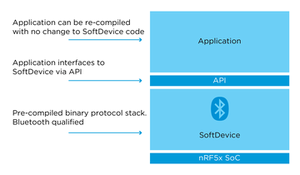
\includegraphics[scale=3.0]{images/SoC-Architecture_large.png}
        		\caption{Các lớp trong một chương trình}
        	\end{center}
        \end{figure}
        \subsection{nRFgo Studio}
        nRFgo Studio là chương trình dùng để nạp Softdevice cho các KIT phát triển, hỗ trợ nhiều chức năng liên quan đến Bluetooth, hiển thị trạng thái bộ nhớ hiện tại của chip,... 
        \subsection{Nordic Mesh SDK}
        Trong đề tài này, nhóm sử dụng nRF5 SDK for Mesh phiên bản v1.0.1 vì đây là phiên bản mới nhất vào thời điểm bắt đầu thực hiện luận văn. Ở thời điểm báo cáo luận văn thì Nordic đã cho ra mắt phiên bản v2.0.1 với một số thay đổi như: thêm chức năng provisioning thông qua GATT (PB-GATT), hỗ trợ chức năng Proxy cho các node và đặc biệt nhất: Mesh stack chính thức hoạt động ổn định. \\
        
        Ngoài ra còn có một số tính năng mà Nordic đang và sẽ cung cấp trong SDK này. Lưu ý: Một số tính năng chưa được hiện thực trong phiên bản SDK hiện tại.
            \begin{itemize}
                \item Device State Manager (DSM): DSM lưu trữ vào bộ nhớ flash những thông tin như Network key của mạng hiện tại, địa chỉ của các element,... Sau khi quá trình provisioning cho node mới hoàn tất, DSM sẽ lưu trữ thêm các thông tin của model, bao gồm địa chỉ và key để các model khác có thể giao tiếp với model này.
                \item Device Firmware Update (DFU): DFU giúp lập trình viên cập nhật firmware cho tất cả node trong mạng mà không cần tiếp xúc trực tiếp với từng node bằng cách áp dụng khả năng lan truyền của mesh.
                \item Hỗ trợ kết nối GATT/GAP, liên kết mạng mesh với các thiết bị như máy tính, điện thoại thông minh,...
                \item Serial, RTT: Cung cấp kênh giao tiếp giữa chip và máy tính, có thể truyền lệnh hay dữ liệu qua lại.
            \end{itemize}
            
        \subsection{Nordic SDK}
        SDK này cung cấp các API để người lập trình dễ dàng lập trình trên các dòng chip của Nordic, cụ thể là chip nRF52832 trong đề tài này. Tuy nhiên do phát triển không đồng thời với Mesh SDK nên khi sử dụng chung có thể gây ra xung đột, đặc biệt là các ứng dụng có dùng Softdevice vì đa phần các API của Nordic SDK không tương thích với Softdevice. Nhóm sử dụng Nordic nRF5 SDK v14.2.0\cite{nrf5sdk}.
    	\subsection{Thư viện giao tiếp module SIM}
    	Thư viện do nhóm tự phát triển và sử dụng trong một dự án trước đây, nhằm mục đích giao tiếp với module 3G SARA click. Thư viện có sẵn một số API cung cấp chức năng cơ bản như: khởi tạo, nghe gọi, xử lý tin nhắn, GPRS, HTTP request,... Trong đề tài này nhóm hiện thực thêm phần giao tiếp TCP để kết nối với cloud.
    	\subsection{ThingSpeak}
    	Nhóm sử dụng một cloud thông dụng dành cho các ứng dụng IoT giám sát đơn giản là ThingSpeak. Dữ liệu sau khi upload lên sẽ được hiển thị dạng biểu đồ và bất kỳ ai có liên kết đều có thể quan sát.
    	\subsection{Embedded Studio}
    	Chương trình hoàn toàn miễn phí, đóng vai trò IDE được Nordic khuyên dùng, các ví dụ được cung cấp trong các SDK đều được viết dưới dạng 1 project Segger Embedded Studio. Đặc biệt các project này đã cấu hình sẵn địa chỉ nạp để tránh đụng độ với Softdevice.
    \section{Mô hình thiết kế}
    Nhóm sử dụng 3 node, 1 node client đóng vai trò gateway, 2 node server đóng vai trò node cảm biến, trong đó node nằm giữa có thêm chức năng node relay. Node gateway sẽ gieo tiếp với node cảm biến xa nhất thông qua node relay. Dữ liệu cảm biến sẽ đọc từ cảm biến nhiệt on board - dùng để đo nhiệt độ hoạt động của SoC.
    \begin{figure}[h!]
    	\begin{center}
    		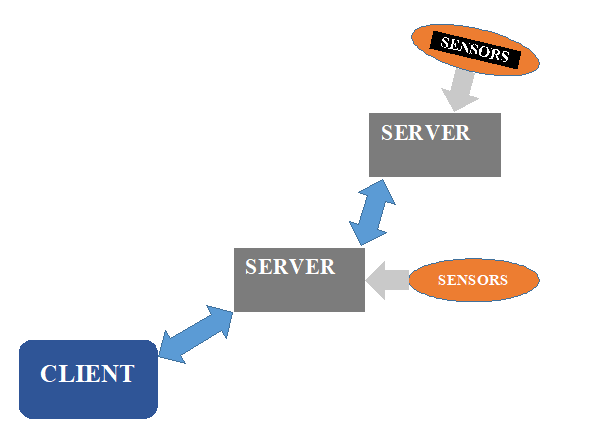
\includegraphics[scale=0.7]{images/design-model.png}
    		\caption{Mô hình thiết kế}
    	\end{center}
    \end{figure}
    

\chapter{Hiện thực ứng dụng}
    \section{Chỉnh sửa model Simple OnOff}\label{simpleonoff}
        \subsection{Model Simple OnOff}
        Trong Mesh SDK v1.0.1 của Nordic có cung cấp sẵn một model là Simple OnOff, cho phép gửi/nhận một 1 bit. Node gateway có thể gửi tín hiệu để tắt mở LED trên node cảm biến bằng hàm set, cũng như dùng hàm get để yêu cầu node cảm biến gửi trạng thái hiện tại của LED cho mình.
        \subsection{Khó khăn}
        Tuy nhiên vì mục đích chỉ là một ví dụ cho người dùng làm quen với cách lập trình sử dụng SDK nên cách hoạt động của model Simple OnOff cũng rất đơn giản, nếu muốn sử dụng model này vào trong đề tài, buộc nhóm phải chỉnh sửa lại model này hoặc tạo một model mới. Nhóm đã tham khảo trong tài liệu của Bluetooth Mesh, cụ thể là Mesh Model Specification 1.0 \cite{meshspec}, phát hiện SIG có định nghĩa một model Sensor với đầy đủ các thuộc tính ID, chu kỳ, hàm đọc giá trị,... nghĩa là trong tương lai Mesh SDK sẽ hỗ trợ model này. Do đó việc tạo một model mới để đọc giá trị cảm biến là không cần thiết, nhóm sẽ chỉnh sửa model Simple OnOff để phục vụ đề tài.
        \subsection{Thực hiện}
        Việc can thiệp vào model Simple OnOff đòi hỏi nhóm phải đọc mã nguồn và tìm ra những điểm liên quan đến gói tin giao tiếp của model này. Kiểu dữ liệu của gói tin được định nghĩa trong file simple\_on\_off\_common.h, còn các hàm liên quan đến việc get/set có trong file simple\_on\_off\_client.h và simple\_on\_off\_server.h, nhóm chỉnh sửa các kiểu dữ liệu để đồng bộ với nhau và model này đã có thể gửi những dữ liệu với kích thước lớn hơn, giới hạn là 10 bytes cho gói đơn lẻ, 384 bytes cho gói fragmented (chia nhỏ gói tin để gửi nhiều lần, sau đó ghép lại)\cite{nordiccase125876}. Sở dĩ có giới hạn này là Bluetooth Mesh sử dụng sóng radio, mà gói tin nhỏ sẽ giúp giảm bớt đụng độ, giới hạn 10 bytes đã được tính toán đủ cho một số ứng dụng thông thường.
    \section{Kết hợp thư viện SDK common}
        \subsection{Khó khăn}
        Việc hiện thực ứng dụng đòi hỏi phải có timer để xử lý các chu kỳ, UART để giao tiếp với module SIM (khác với UART dùng để giao tiếp với máy tính), nhưng Mesh SDK lại không hỗ trợ hai thư viện này mà chỉ có một thư viện hal (Hardware abstract layer) rất khó sử dụng. Do đó nhóm cần phải kết hợp Mesh SDK với SDK common của Nordic cung cấp để lập trình trên kit phát triển của hãng, phiên bản dùng trong đề tài là nRF5\_SDK\_14.2.0\cite{nrf5sdk}.
        \subsection{Thực hiện}
        Nhóm thử tiến hành kết hợp bằng 2 hướng tiếp cận:
        \begin{itemize}
            \item Chép các file từ common SDK sang mesh SDK: không thành công vì xuất hiện rất nhiều lỗi liên quan đến việc liên kết giữa các header và file mã nguồn nhưng vì số lượng file quá nhiều nên không sửa hết các liên kết này.
            \item Chép các file từ mesh SDK sang common SDK, hướng này cũng là hướng dẫn của chính Nordic: không thành công vì khi liên quan đến softdevice, một số drivers của common SDK bị xung đột.
        \end{itemize}
        Sau đó, nhóm sử dụng giải pháp chép các file từ common SDK sang mesh SDK nhưng không phải toàn bộ mà chép từng phần. Nếu cần dùng UART thì chép những file liên quan đến UART, cần dùng Timer thì chép file liên quan đến Timer và cách này đã hoạt động tốt.
    \section{Hiện thực node cảm biến}
        \subsection{Đọc giá trị cảm biến}
        Node cảm biến không thực hiện thêm chức năng gì so với mã nguồn mẫu ban đầu của SDK, chỉ chỉnh sửa hàm get\_cb (được kích hoạt khi node gateway gửi yêu cầu đọc dữ liệu cảm biến) để hàm trả về giá trị cảm biến hiện tại. Việc đọc giá trị cảm biến được softdevice hỗ trợ sẵn với hàm sd\_temp\_get().
    \section{Hiện thực node gateway}
        \subsection{Thư viện giao tiếp với module SIM}
        Thư viện này nhóm viết bằng ngôn ngữ C++ mà cả common SDK và mesh SDK đều dùng C, nên khi sử dụng trong đề tài này đã gặp phải khó khăn: không compile được. Nhóm phát triển dựa trên mã nguồn và file Segger Embedded Studio nên mọi thông số mặc định đều dành cho ngôn ngữ C, cách giải quyết lại chỉnh sửa thư viện của nhóm để phù hợp với compiler.


\chapter{Kịch bản thử nghiệm} \label{chap:experiment}
    \section{Mục tiêu của thử nghiệm}
    \begin{itemize}
        \item Kiểm tra hoạt động của ứng dụng: node gateway thu thập dữ liệu từ các node cảm biến sau đó gửi lên cloud, ấn nút trên node gateway để điều khiển LED trên các node cảm biến.
        \item Chứng minh ứng dụng được hiện thực bằng giao thức mạng Mesh, cụ thể là vai trò của node relay.
        \item Chứng minh các node trong mạng có thể giao tiếp với nhau bằng cả 2 chiều gửi và nhận: node cảm biến gửi dữ liệu cho node gateway và nhận tín hiệu bật/tắt LED từ node gateway.
        \item Kiểm tra khoảng cách hoạt động tối đa giữa các node.
    \end{itemize}
    \section{Quá trình thử nghiệm}
        Nhóm thử nghiệm với 3 board phát triển, một board là node gateway còn lại là node cảm biến lần lượt gọi là node 0 và node 1. Đầu tiên cần tiến hành provision cho 2 node cảm biến: chỉ cần bật nguồn node gateway trước, rồi lần lượt bật nguồn node 0 và node 1. Sau đó tiến hành thử nghiệm bằng các kịch bản sau:
        \subsection{Kịch bản I: Thử nghiệm giao tiếp}
        \begin{itemize}
            \item Đặt 2 node 0 và node 1 ở gần node gateway, sau đó thử ấn nút gửi tín hiệu điều khiển LED thì thấy LED trên cả 2 node cảm biến chớp tắt.
            \begin{figure}[h!]
	    	 \begin{center}
	    		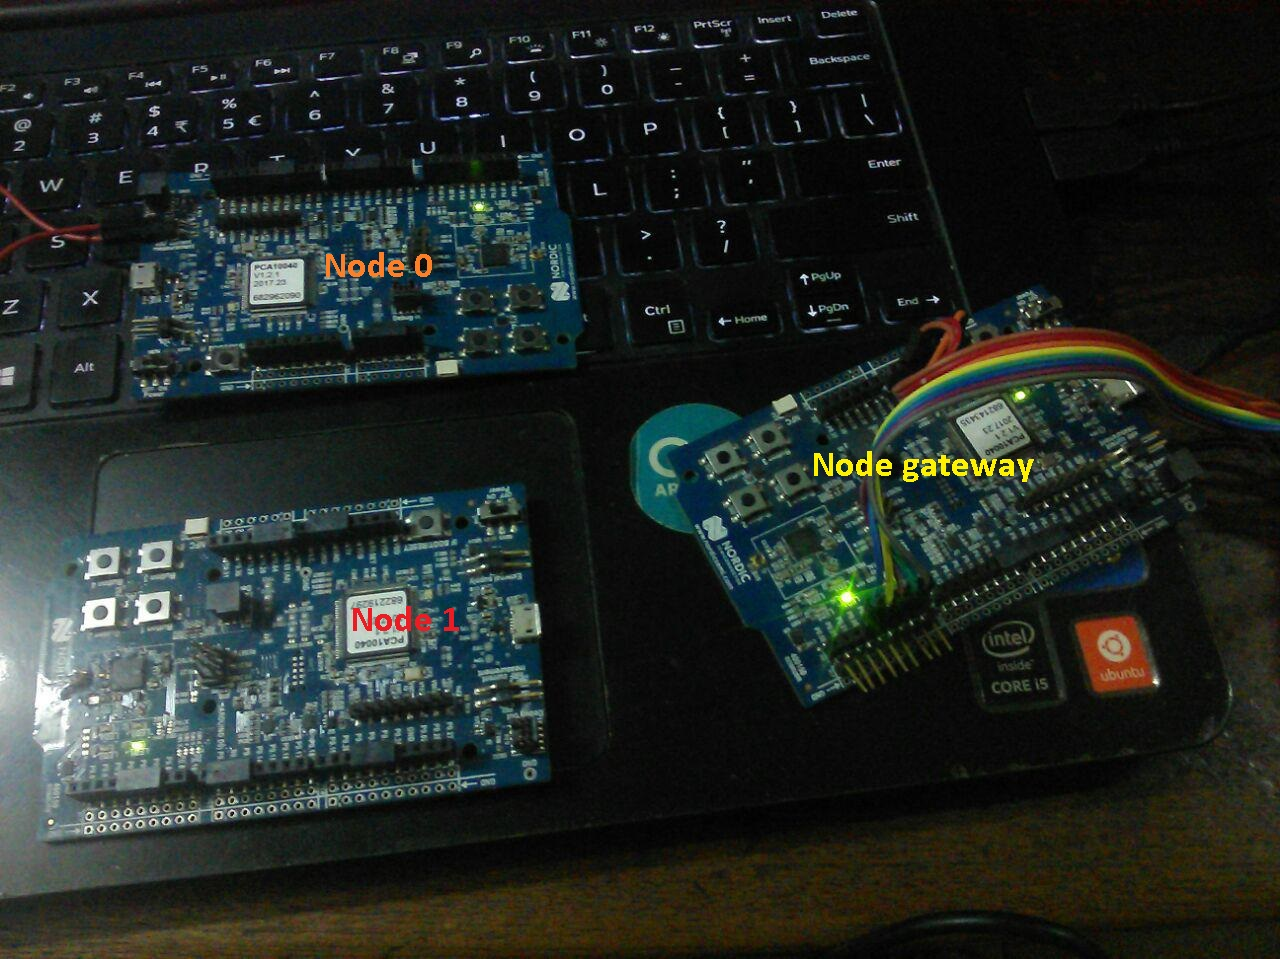
\includegraphics[scale=0.4]{images/ex1-1.jpg}
	    		\caption{Hình ảnh thử nghiệm I trong thực tế}
	    	\end{center}
    	\end{figure}
            \item Sau đó thử kích hoạt chế độ đọc và gửi dữ liệu cảm biến thì thấy node gateway nhận được dữ liệu và gửi lên server thành công. Có thể thử thay đổi dữ liệu bằng cách tăng nhiệt độ ở khu vực gần SoC nRF52832 trên Kit phát triển.
            \begin{figure}[h!]
	    	 \begin{center}
	    		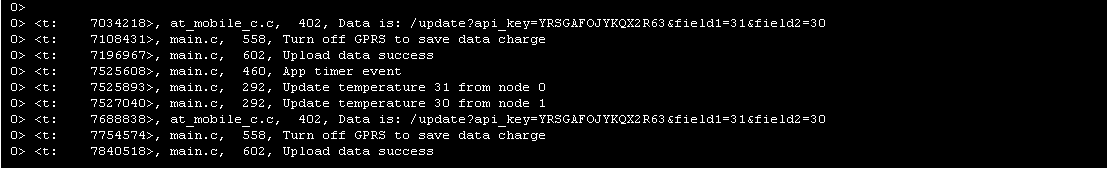
\includegraphics[scale=0.4]{images/ex1-2.png}
	    		\caption{Hình ảnh note gateway nhận được dữ liệu từ node cảm biến}
	    	\end{center}
    	\end{figure}
    	\begin{figure}[h!]
	    	 \begin{center}
	    		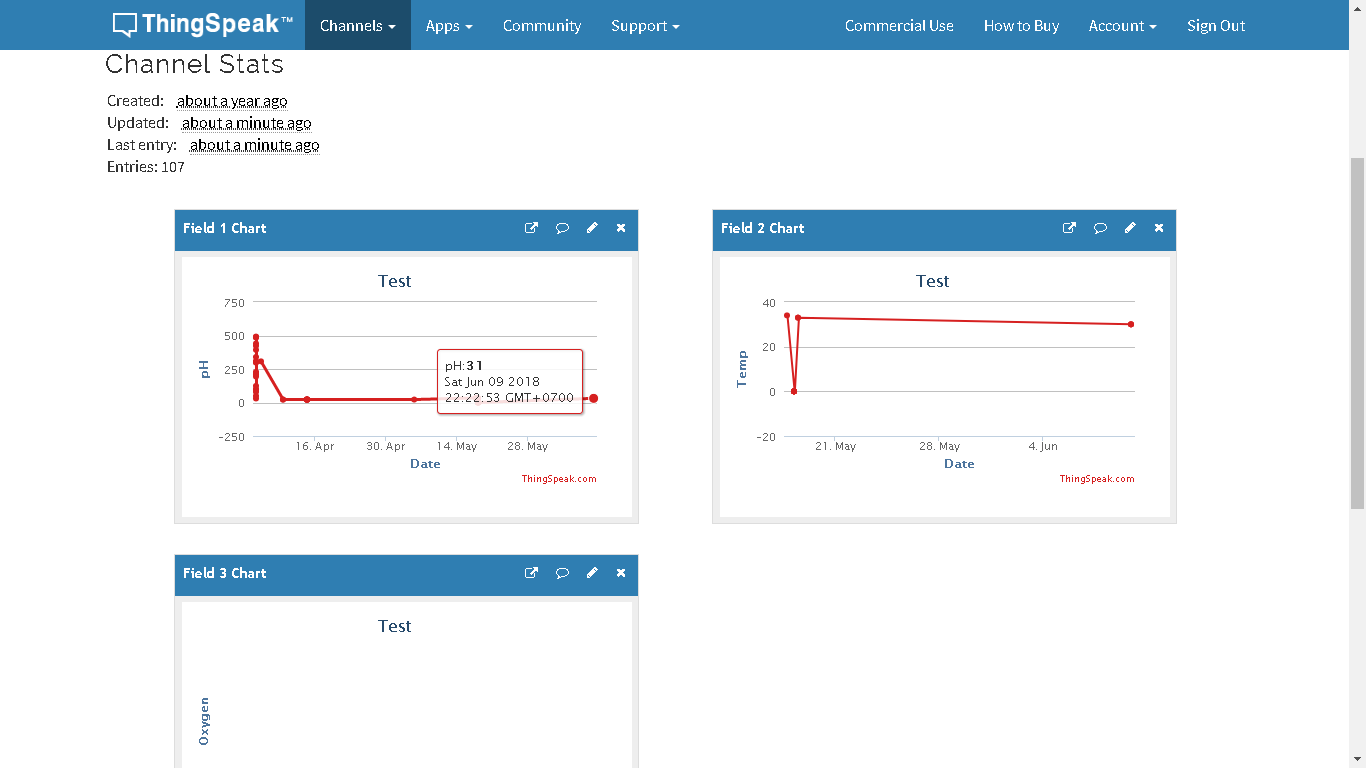
\includegraphics[scale=0.4]{images/ex1-3.png}
	    		\caption{Hình ảnh dữ liệu được cập nhật lên cloud}
	    	\end{center}
    	\end{figure}
            \item Thử tắt nguồn node 0 thì thấy node gateway báo lỗi không đọc được dữ liệu từ node 0, khi bật nguồn lại thì hoạt động bình thường trở lại.
        \end{itemize}
        \textbf{Kết quả thử nghiệm của kịch bản I chứng minh khả năng hoạt động của ứng dụng khi không có lỗi phát sinh.}
        \subsection{Kịch bản II: Thử nghiệm khoảng cách}
        \begin{itemize}
            \item Tiến hành với một node gateway và một node cảm biến là node 0, node gateway sẽ gửi lệnh điều khiển LED liên tục bằng cách nhấn nút.
            \item Sau đó dời node cảm biến dần dần ra xa cho đến khi LED trên node cảm biến không còn chớp tắt nữa thì dừng lại.
            \begin{figure}[h!]
	    	 \begin{center}
	    		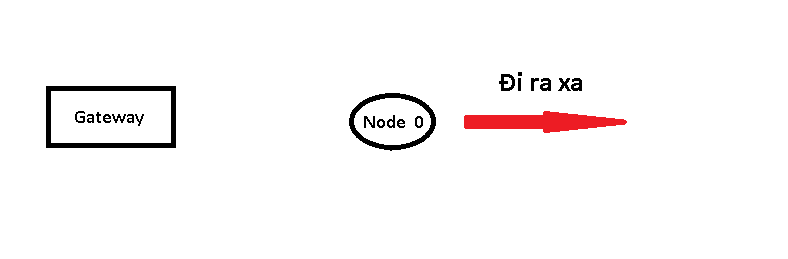
\includegraphics[scale=0.8]{images/ex2-1.png}
	    		\caption{Hình ảnh thử nghiệm II trong thực tế}
	    	\end{center}
        	 \end{figure}
            \item Khoảng cách giữa node gateway và node 0 lúc này là khoảng cách tối đa giữa 2 node của Bluetooth Mesh. Sau đó dời node 0 ra xa thêm khoảng 2m để tiến hành thử kịch bản III.
        \end{itemize}
        \textbf{Kết quả thử nghiệm của kịch bản II chứng tỏ khoảng cách giao tiếp tối đa giữa 2 node trong thực tế (không có vật cản) là khoảng từ 8-10m.}
        \subsection{Kịch bản III: Thử nghiệm truyền dữ liệu trong mạng mesh}
        \begin{figure}[h!]
	    	 \begin{center}
	    		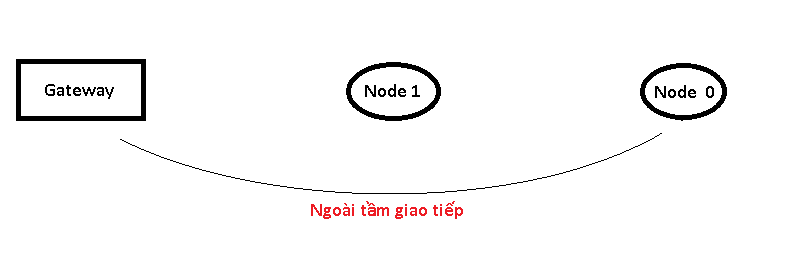
\includegraphics[scale=0.8]{images/ex3-1.png}
	    		\caption{Hình ảnh thử nghiệm III}
	    	\end{center}
        \end{figure}
        \begin{itemize}
            
            \item Sau khi node 0 đã nằm ngoại phạm vi giao tiếp với node gateway, đặt node 1 vào khoảng giữa 2 node này.
            \begin{figure}[h!]
	    	 \begin{center}
	    		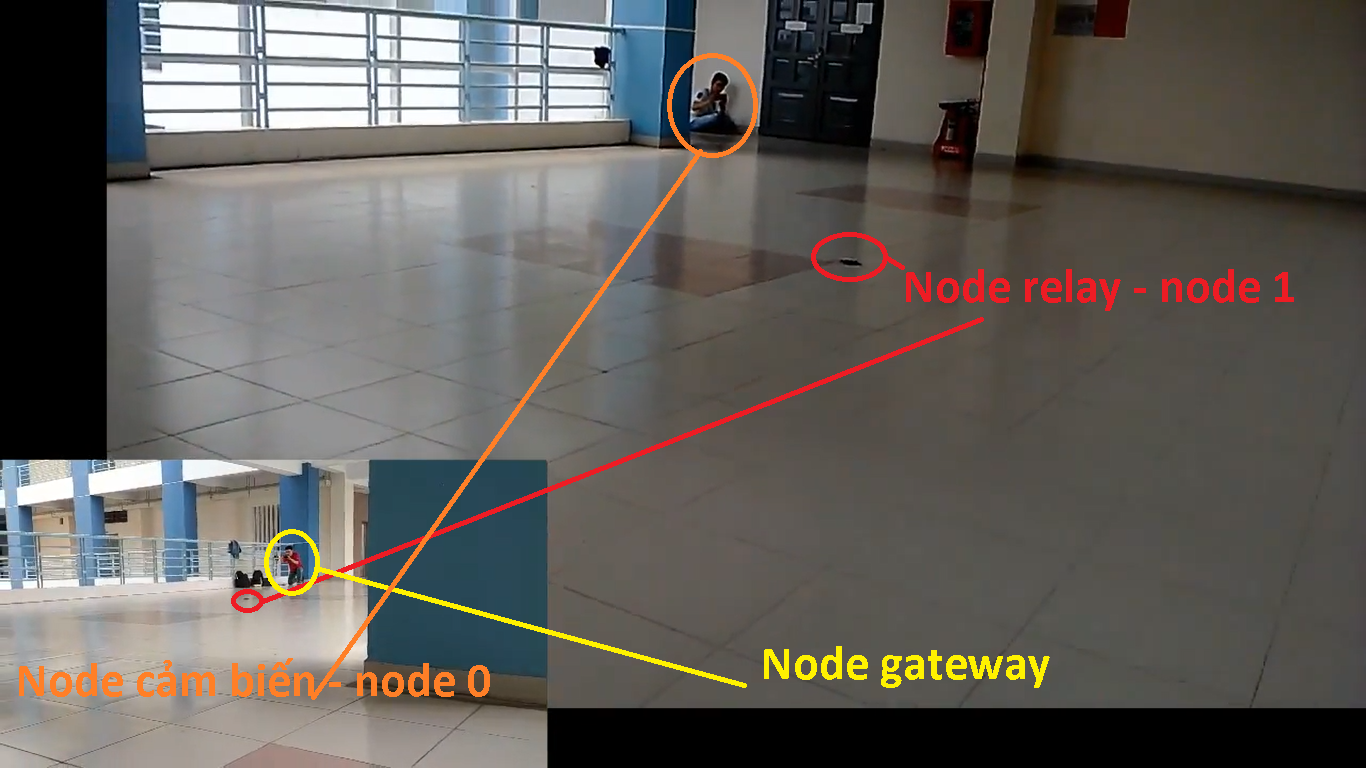
\includegraphics[scale=0.3]{images/ex3-2.png}
	    		\caption{Hình ảnh thử nghiệm III trong thực tế}
	    	\end{center}
    	\end{figure}
    	\newpage
            \item Sau đó tiến hành gửi tín hiệu điều khiển LED bằng node gateway, lúc này LED trên cả node 0 lẫn node 1 đều chớp tắt, chứng tỏ tín hiệu đã được node 1 relay lại và node 0 đã nhận được tín hiệu điều khiển (tín hiệu này gửi multicast nên cả 2 node 0 và 1 đều chớp LED).
            \begin{figure}[h!]
	    	 \begin{center}
	    		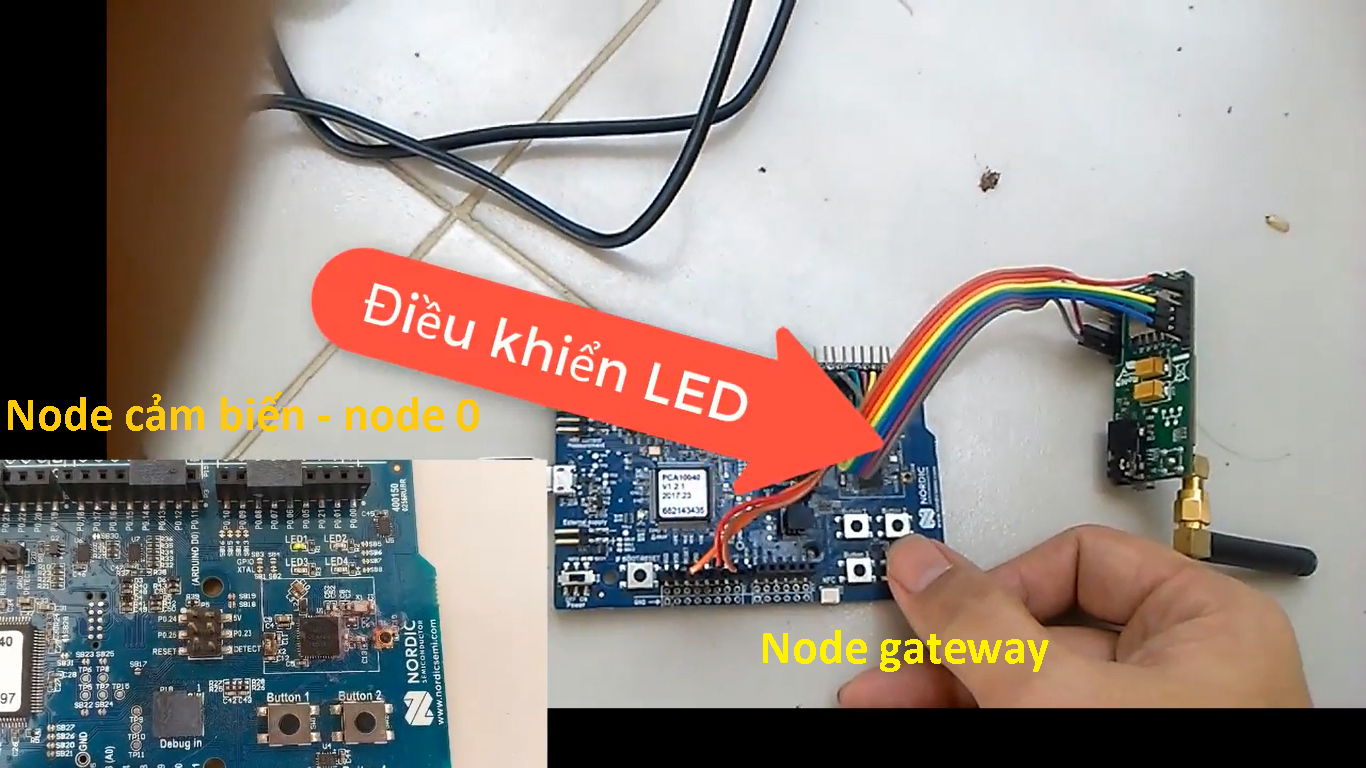
\includegraphics[scale=0.3]{images/ex3-3.png}
	    		\caption{Hình ảnh điều khiển LED trong thực tế}
	    	\end{center}
    	\end{figure}
        \end{itemize}
        \textbf{Kết quả thử nghiệm của kịch bản III chứng tỏ rằng node 1 đã đóng vai trò relay, giúp chuyển tiếp dữ liệu từ node gateway đến cho node 0.}






\chapter{Kết luận}\label{chap:conclude}
    \section{Đánh giá kết quả}
    	\subsection{Thành quả đạt được}
    	
    \begin{itemize}
        \item Tổng kết thành quả của nhóm trong quá trình nghiên cứu lý thuyết về Bluetooth Mesh: nguyên nhân ra đời, tiềm năng cạnh tranh, sơ lược về các lớp trong kiến trúc, cách truyền nhận dữ liệu giữa các node trong mạng, cách quản lý việc kết nối/ngắt kết nối.
        \item Kết quả nghiên cứu có thể được dùng làm tài liệu tham khảo cho những ai muốn làm quen với Bluetooth Mesh, giúp tiết kiệm thời gian tiếp cận.
        \item Hiện thực thành công ứng dụng sử dụng giao thức Bluetooth Mesh để giao tiếp. Mặc dù ứng dụng chưa quá hoàn thiện để có thể đưa vào thực tế, tuy nhiên cũng chứng minh được dữ liệu có thể đi theo 2 chiều gửi và nhận.
    \end{itemize}
    
    \subsection{Một số hạn chế của ứng dụng thử nghiệm}
    \begin{itemize}
        \item Chưa hỗ trợ thiết lập các thông số một cách linh hoạt: chu kỳ đọc, chu kỳ gửi, thông số cloud,...
        \item Chưa hỗ trợ lấy thông tin thiết bị
        \item Chưa hỗ trợ xóa node khỏi mạng
        \item Chưa hỗ trợ cơ chế xác thực mạnh khi provisioning
    \end{itemize}
    \section{Hướng phát triển}
    Do không đủ nhân lực nên nhóm chưa hiện thực tốt ứng dụng thử nghiệm, tuy nhiên nhóm có đề xuất một số cải tiến để ứng dụng thử nghiệm có thể trở thành ứng dụng trong thực tế:
    
    \begin{itemize}
        \item Tăng khả năng bảo mật bằng cách tăng giảm thông số node cảm biến tối đa trong mạng thông qua node gateway. Ví dụ hiện đang có 2 node cảm biến trong mạng, thông số node tối đa là 2, node cảm biến tiếp theo muốn tham gia vào mạng phải chờ node gateway tăng thông số node tối đa lên mới tham gia được. Bước này giúp tránh việc có node cảm biến tình cờ có được key vào mạng liền vào mạng với ý định xấu.
        \item Hiện thực giao diện cho node gateway để dễ dàng tiến hành các thao tác cấu hình như: thiết lập chu kỳ đọc dữ liệu, chu kỳ gửi dữ liệu, địa chỉ remote server, số node cảm biến tối đa, xóa node cảm biến ra khỏi mạng,...
        \item Hiện thực giao diện người dùng lấy dữ liệu từ remote server.
        \item Hiện thức một giao thức giao tiếp giữa các node để tránh tình trạng nghẽn mạng, quy trình xử lý khi node gateway mất kết nối hoặc node cảm biến mất kết nối.
    \end{itemize}
    
    \subsection{Tiềm năng trong thực tế}
    \begin{itemize}
        \item Hệ thống đèn lớn: Yêu cầu chính của hệ thống này là một bộ điều khiển có thể điều khiển một nhóm (có thể là cùng một tầng hoặc cùng một phòng) hay toàn bộ đèn, Bluetooth Mesh cực kỳ thích hợp trong ứng dụng này. Chỉ với một node client điều khiển và hàng ngàn node server với tốc độ đáp ứng nhanh, chức năng điều khiển đơn giản chỉ là bật tắt - thậm chí trong tương lai model này còn hỗ trợ độ mạnh yếu của đèn - là hệ thống có thể hoạt động tốt.
        \item Hệ thống cảm biến lớn: Những hệ thống như dây chuyền sản xuất tự động trong công nghiệp đòi hỏi có rất nhiều cảm biến đặt rải rác ở nhiều khâu trên dây chuyền. Tất cả các cảm biến đó sẽ gửi toàn bộ thông tin về một node trung tâm, sau đó node trung tâm này sẽ gửi 1 loạt dữ liệu đó lên server hoặc lưu vào một loại database nào đó, vì số lượng cảm biến trong hệ thống rất nhiều nên nếu mỗi node mỗi gửi dữ liệu sẽ dẫn đến một cuộc "DoS" nhẹ!
        \item Hệ thống theo dõi trong nhà: Rất nhiều cảm biến GPS hiện nay tín hiệu không đủ mạnh để định vị trong nhà, đặc biệt là ở tầng thấp. Bluetooth Mesh có thể khắc phục điểm yếu đó và kết hợp tốt với GPS, chúng ta có thể dựa vào mức độ mạnh yếu của tín hiệu và áp dụng thêm các thuật toán để xác định vị trí cũng như độ cao cụ thể của người hay vật trong nhà với độ chính xác cao.
    \end{itemize}
%\include{main/experiment}
%\include{main/conclusion}


%%%%%%%%%%%%%%%%%%%%%%%%%%%%%%%%%%%%%%%%%%%%%%
%%%%% TAIL: Bibliography, Appendix, CV
%%%%%%%%%%%%%%%%%%%%%%%%%%%%%%%%%%%%%%%%%%%%%%
\appendix
\chapter{Một số Model chuẩn}\label{models}

\section{Foundation models}
Foundation models have been defined in the core specification. Two of them are mandatory for all mesh nodes.

\begin{itemize}
	\item Configuration Server (mandatory)
	\item Configuration Client
	\item Health Server (mandatory)
	\item Health Client
\end{itemize}

\section{Generic models}
\begin{itemize}
\item Generic OnOff Server, used to represent devices that do not fit any of the model descriptions defined but support the generic properties of On/Off
\item Generic Level Server, keeping the state of an element in a 16-bit signed integer
\item Generic Default Transition Time Server, used to represent a default transition time for a variety of devices
\item Generic Power OnOff Server \& Generic Power OnOff Setup Server, used to represent devices that do not fit any of the model descriptions but support the generic properties of On/Off
\item Generic Power Level Server \& Generic Power Level Setup Server, including a Generic Power Actual state, a Generic Power Last state, a Generic Power Default state and a Generic Power Range state
\item Generic Battery Server, representing a set of four values representing the state of a battery
\item Generic Location Server \& Generic Location Setup Server, representing location information of an element, either global (Lat/Lon) or local
\item Generic User/Admin/Manufacturer/Client Property Server, representing any value to be stored by an element
\item Generic OnOff Client \& Generic Level Client
\item Generic Default Transition Time Client
\item Generic Power OnOff Client \& Generic Power Level Client
\item Generic Battery Client
\item Generic Location Client
\item Generic Property Client
\end{itemize}

\section{Sensors}
\begin{itemize}
\item Sensor Server \& Sensor Setup Server, representing a sensor device. Sensor device may be configured to return a measured value periodically or on request; measurement period (cadence) may be configured to be fixed or to change, so that more important value range is being reported faster.
\item Sensor Client
\end{itemize}

\section{Time and scenes}
\begin{itemize}
\item Time Server \& Time Setup Server, allowing for time synchronization in mesh network
\item Scene Server \& Scene Setup Server, allowing for up to 65535 scenes to be configured and recalled when needed.
\item Scheduler Server \& Scheduler Setup Server
\item Time Client, Scene Client \& Scheduler Client
\end{itemize}

\section{Lighting}
\begin{itemize}
\item Light Lightness Server \& Light Lightness Setup Server, representing a dimmable light source
\item Light CTL Server, Light CTL Temperature Server \& Light CTL Setup Server, representing a CCT or "tunable white" light source
\item Light HSL Server, Light HSL Hue Server, Light HSL Saturation Server \& Light HSL Setup Server, representing a light source based on Hue, Saturation, Lightness color representation
\item Light xyL Server \& Light xyL Setup Server, representing a light source based on modified CIE xyY color space.
\item Light LC (Lightness Control) Server \& Light LC Setup Server, representing a light control device, able to control Light Lightness model using an occupancy sensor and ambient light sensor. It may be used for light control scenarios like Auto-On, Auto-Off and/or Daylight Harvesting.
\item Light Lightness Client, Light CTL Client, Light HSL Client, Light xyL Client \& Light LC Client
\end{itemize}

\chapter{Flowchart quá trình remote provisioning}\label{remoteprov}
    \begin{figure}[h!]
    	\begin{center}
    		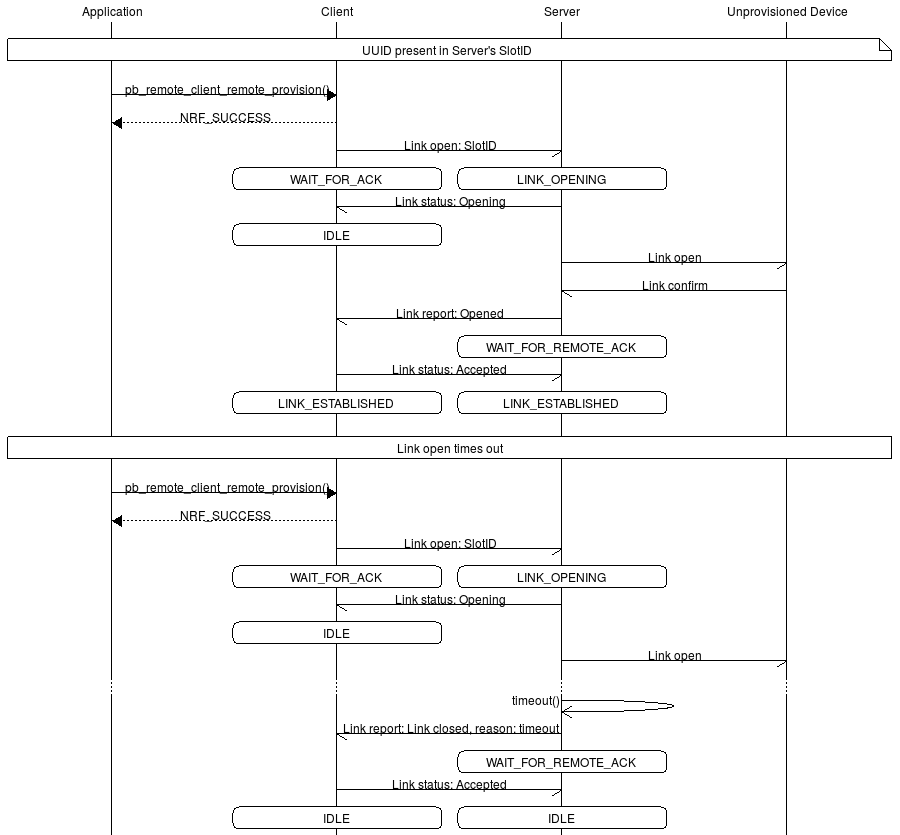
\includegraphics[scale=0.4]{images/msc_pb_remote_link_open.png}
    		\caption{Quá trình remote provisioning}
    	\end{center}
    \end{figure}
    
\chapter{Hướng dẫn thực thi ứng dụng}\label{guide}
\begin{enumerate}
\item Sau khi kết nối Kit PCA10040 với máy tính, sử dụng phần mềm nRFgo Studio để nạp Softdevice cho Kit.
            \begin{figure}[h!]
    	 \begin{center}
    		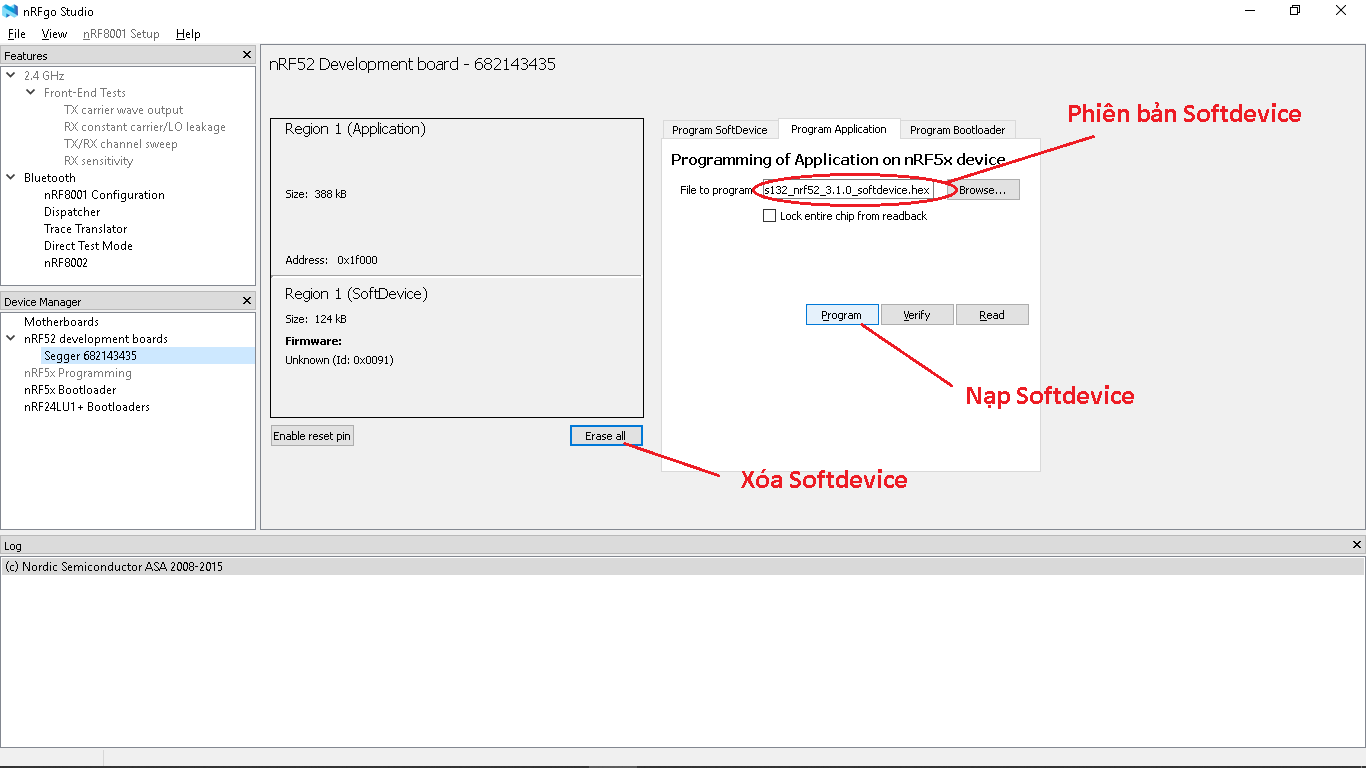
\includegraphics[scale=0.4]{images/app3-1.png}
    		\caption{Giao diện phần mềm nRFgo Studio}
    	\end{center}
    	\end{figure}
\item Sau khi đã nạp Softdevice, tiến hành nạp các chương trình khác nhau cho node cảm biến và node gateway. Node cảm biến sẽ dùng project - Embedded Studio Project - server còn node gateway sẽ dùng project client.
            \begin{figure}[h!]
    	 \begin{center}
    		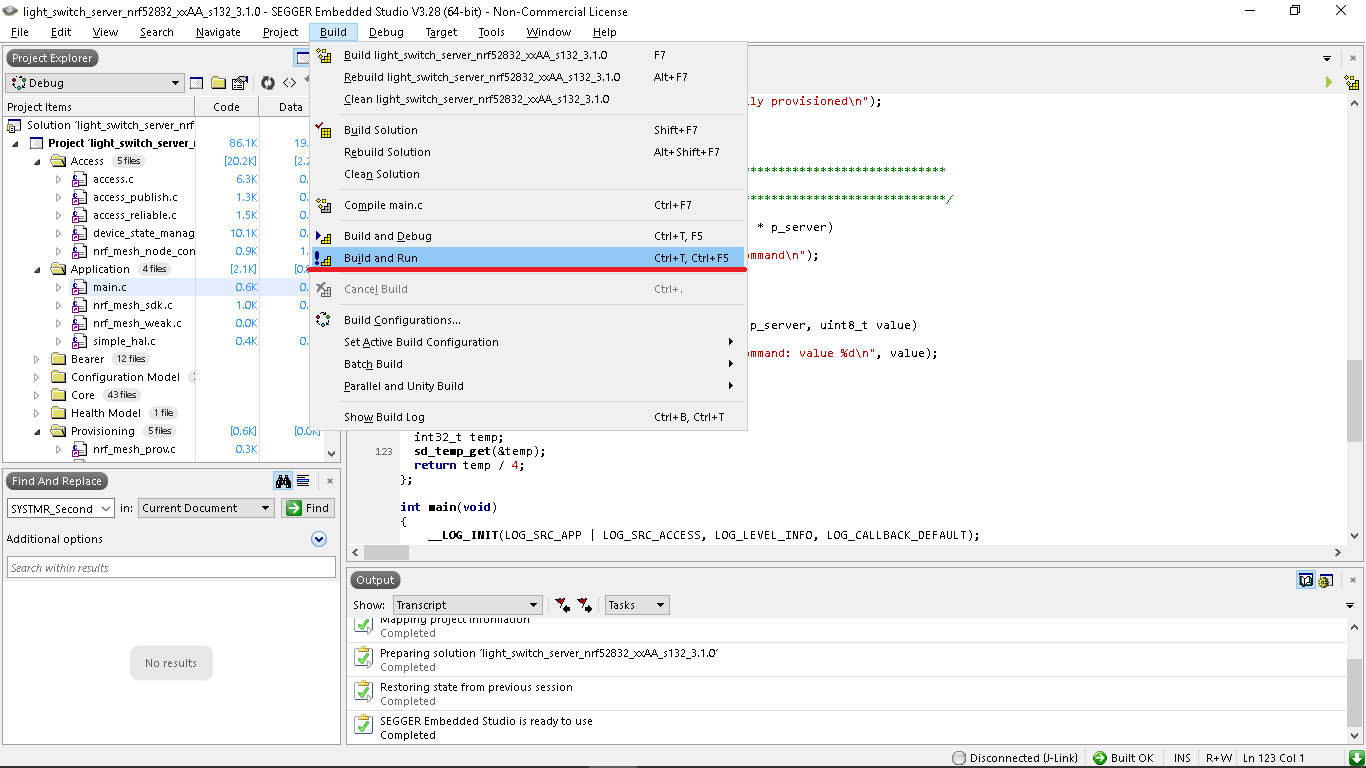
\includegraphics[scale=0.4]{images/app3-2.png}
    		\caption{Giao diện phần mềm Embedded Studio Project}
    	\end{center}
    	\end{figure}
    	\newpage
\item Để theo dõi quá trình thực thi của chương trình, sử dụng J-link RTT Viewer để xem quan sát quá trình.
	 \begin{figure}[h!]
    	 \begin{center}
    		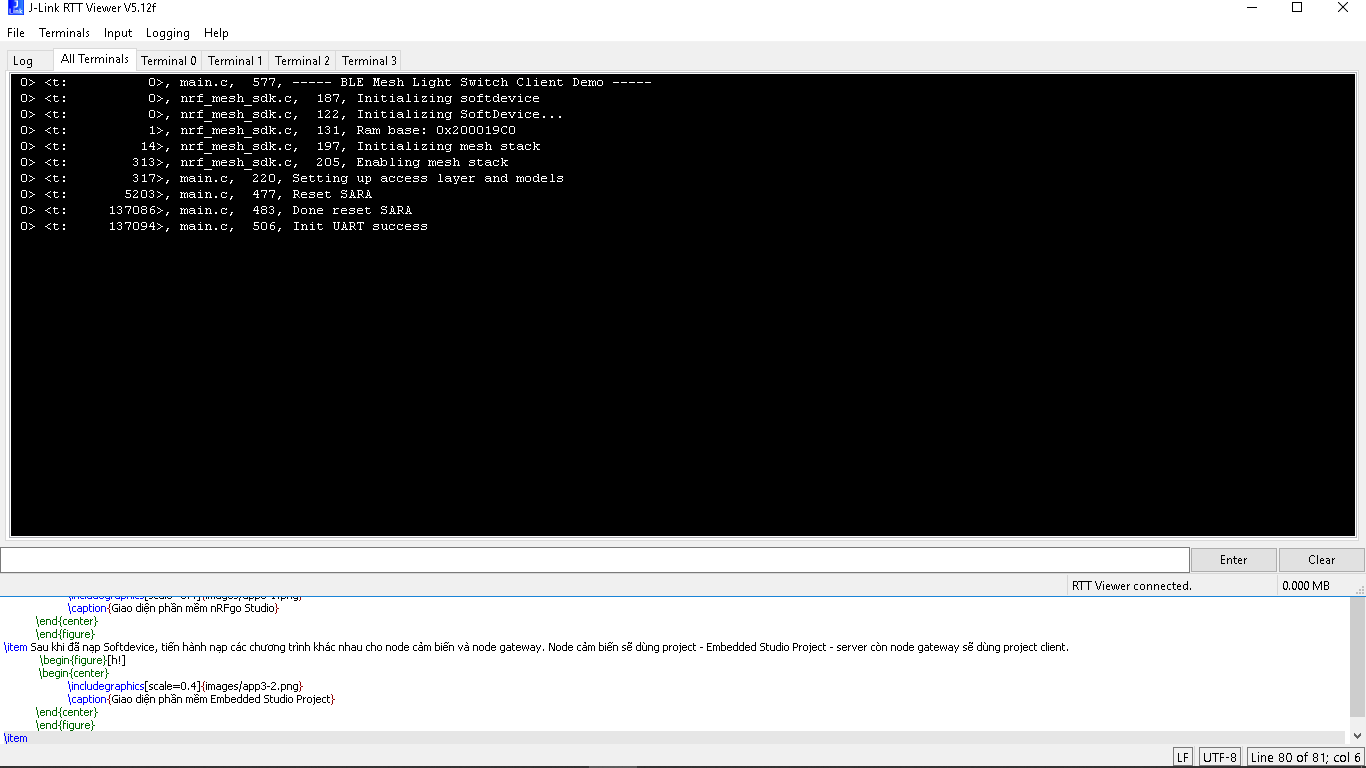
\includegraphics[scale=0.4]{images/app3-3.png}
    		\caption{Giao diện phần mềm J-link RTT Viewer}
    	\end{center}
    	\end{figure}
\end{enumerate}
\backmatter
\cleardoublepage
\renewcommand{\bibname}{Tài liệu tham khảo}
\begin{thebibliography}{80}

%[1]
\bibitem{cmcn}
Cách mạng Công nghiệp 4.0 là gì?
\\\texttt{\url{https://news.zing.vn/cach-mang-cong-nghiep-40-la-gi-post750267.html}}

%[2]
\bibitem{meshadvan}
Implementing a mesh network? Here’s why you should use Bluetooth
\\\texttt{\url{http://www.embedded-computing.com/iot/implementing-a-mesh-network-here-s-why-you-should-use-bluetooth}}

%[3]
\bibitem{meshborn}
Bluetooth SIG Announces Mesh Networking Capability
\\\texttt{\url{https://www.bluetooth.com/news/pressreleases/2017/07/bluetooth-sig-announces-mesh-networking-capability}}

%[4]
\bibitem{meshconcept}
Basic Bluetooth Mesh concepts
\\\texttt{\url{http://infocenter.nordicsemi.com/index.jsp?topic=\%2Fcom.nordic.infocenter.meshsdk.v1.0.1\%2Fmd\_doc\_introduction\_basic\_concepts.html\&cp=4\_1\_0\_0\_0}}

%[5]
\bibitem{ECDH}
Elliptic-curve Diffie–Hellman
\\\texttt{\url{https://en.wikipedia.org/wiki/Elliptic-curve\_Diffie\%E2\%80\%93Hellman}}

%[6]
\bibitem{meshspec}
Mesh Networking Specifications
\\\texttt{\url{https://www.bluetooth.com/specifications/mesh-specifications}}

%[7]
\bibitem{nrf5sdk}
nRF5 SDK
\\\texttt{\url{https://www.nordicsemi.com/eng/Products/Bluetooth-low-energy/nRF5-SDK}}


\bibitem{meshgloss}
Bluetooth Mesh Glossary of Terms
\\\texttt{\url{https://www.bluetooth.com/bluetooth-technology/topology-options/le-mesh/mesh-glossary}}

\bibitem{meshfriend}
Bluetooth Mesh Networking: Friendship
\\\texttt{\url{http://blog.bluetooth.com/bluetooth-mesh-networking-series-friendship}}

\bibitem{meshintro}
A Closer Look at the New Bluetooth Mesh
\\\texttt{\url{https://www.betasolutions.co.nz/Blog/12/A-Closer-Look-at-the-New-Bluetooth-Mesh}}

\bibitem{meshfaq}
Bluetooth Mesh FAQ
\\\texttt{\url{https://www.bluetooth.com/bluetooth-technology/topology-options/le-mesh/mesh-faq}}

\bibitem{meshpart1}
The Fundamental Concepts of Bluetooth Mesh Networking Part 1
\\\texttt{\url{https://blog.bluetooth.com/the-fundamental-concepts-of-bluetooth-mesh-networking-part-1}}

\bibitem{meshsecure}
Bluetooth Mesh Security Overview
\\\texttt{\url{https://blog.bluetooth.com/bluetooth-mesh-security-overview}}


\bibitem{nordiccase125876} 
How to add uart function to light control client demo at nrf5\_SDK\_for\_Mesh\_v0.9.2-Alpha
\\\texttt{\url{https://devzone.nordicsemi.com/f/nordic-q-a/25877/how-to-add-uart-function-to-light-control-client-demo-at-nrf5\_sdk\_for\_mesh\_v0-9-2-alpha}}

\bibitem{softdevice}
S132 SoftDevice
\\\texttt{\url{https://www.nordicsemi.com/eng/Products/S132-SoftDevice}}


\end{thebibliography}
\addcontentsline{toc}{chapter}{Tài liệu tham khảo}


% Add your glossary here
% Add your index here
% Photographic credits (list of pictures&images that have been used with names of the person holding the copyright for them)
%\include{tail/cv}

\end{document}
\grid
